\subsection{Integers}
\frame{\tableofcontents[currentsubsection]}

\begin{frame}
  \frametitle{Integers}
  \begin{itemize}
    \item \cpp\ offers both signed and unsigned integers
    \item For clarity's sake, examples will use 8-bit integers
    \item But same is applicable on 16, 32, 64, \dots bit integers
  \end{itemize}
\end{frame}

\begin{frame}
  \frametitle{Signed Integers}
  \begin{itemize}
    \item MSB is used to represent sign
    \item If MSB = \texttt{0}, then number is positive ($\geq 0$)
    \item If MSB = \texttt{1}, then number is negative ($< 0$)
    \item Java only offers signed integers
  \end{itemize}
  \begin{center}
    \begin{tikzpicture}[scale=0.75,transform shape]
      \draw (0,0) grid (8,1);
      \foreach[evaluate={\i-0.5} as \x] \i in {1,...,8} {
        \tikzmath{
          int \v;
          \v = random(0, 1);
        }
        \node at (\x, 0.5) {\v};
      }
      \draw[|-|] (0,-0.25) -- (1,-0.25) node[midway,below,font=\tiny] {sign bit};
      \draw[|-|] (1,-0.25) -- (8,-0.25) node[midway,below,font=\tiny] {value};
    \end{tikzpicture}
  \end{center}
  \begin{center}
    \begin{tabular}{cccc}
      \toprule
      \textbf{Type} & \textbf{\# Bits} & \textbf{Lowest} & \textbf{Highest} \\
      \midrule
      \texttt{int8\_t} & 8 & $-128$ & $127$ \\
      \texttt{int16\_t} & 16 & \num{-32768} & \num{32767} \\
      \texttt{int32\_t} & 32 & $-2^{31}$ & $2^{31}-1$ \\
      \texttt{int64\_t} & 64 & $-2^{63}$ & $2^{63}-1$ \\
      & $N$ & $-2^{N-1}$ & $2^{N-1}-1$ \\
      \bottomrule
    \end{tabular}
  \end{center}
\end{frame}

\begin{frame}
  \frametitle{Unsigned Integers}
  \begin{itemize}
    \item All bits are used to represent value
  \end{itemize}
  \begin{center}
    \begin{tikzpicture}[scale=0.75,transform shape]
      \draw (0,0) grid (8,1);
      \foreach[evaluate={\i-0.5} as \x] \i in {1,...,8} {
        \tikzmath{
          int \v;
          \v = random(0, 1);
        }
        \node at (\x, 0.5) {\v};
      }
      \draw[|-|] (0,-0.25) -- (8,-0.25) node[midway,below,font=\tiny] {value};
    \end{tikzpicture}
  \end{center}
  \begin{center}
    \begin{tabular}{cccc}
      \toprule
      \textbf{Type} & \textbf{\# Bits} & \textbf{Lowest} & \textbf{Highest} \\
      \midrule
      \texttt{uint8\_t} & 8 & $0$ & $255$ \\
      \texttt{uint16\_t} & 16 & \num{0} & \num{65535} \\
      \texttt{uint32\_t} & 32 & $0$ & $2^{32}-1$ \\
      \texttt{uint64\_t} & 64 & $0$ & $2^{64}-1$ \\
      & $N$ & $0$ & $2^{N}-1$ \\
      \bottomrule
    \end{tabular}
  \end{center}
\end{frame}

\begin{frame}
  \frametitle{Visual Comparison Signed vs Unsigned}
  \begin{center}
    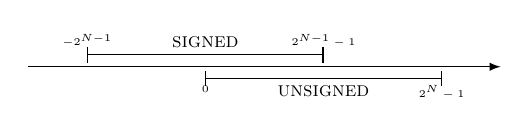
\begin{tikzpicture}[scale=0.75,transform shape]
      \draw[-latex] (-3,0) -- (5,0);

      \draw[|-|] (-2,0.2) -- ++(4,0) node[midway,above] {\bf\sc signed} node[at start,above,font=\tiny] {$-2^{N-1}$} node[at end,above,font=\tiny] {$2^{N-1}-1$};
      \draw[|-|] (0,-0.2) -- ++(4,0) node[midway,below] {\bf\sc unsigned} node[at start,below,font=\tiny] {$0$} node[at end,below,font=\tiny] {$2^N-1$};
    \end{tikzpicture}
  \end{center}
\end{frame}
